\chapter{Realisierung}
\section{Einführung}





\section{User Interface}
\subsection{Allgemein}
In diesem Unterabschnitt werden die Konzepte erklärt, mit welchen das User Interface realisiert wurde. Das Webinterface wurde HTML, CSS und JavaScript erstellt und als unterstützende Library wurde Twitter Bootstrap verwendet.

\subsubsection{Java Server Pages JSP}
Sämtlicher HTML Code ist in Java Server Pages (JSP) abgelegt. JSP Seiten werden auf dem Server in Java Servlets kompiliert.
\begin{figure}[H]
\centering
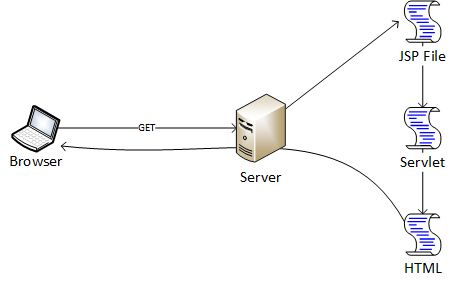
\includegraphics[scale=1]{../04_Realisierung/images/userinterface/jsp.png}
\caption{Java Server Pages}
\end{figure}
Der Client erhält über eine Web-URL vom Server generiertes HTML.

\subsubsection{Java Server Pages Standard Tag Library JSTL}
Mittels JSTL werden in dieser Applikation folgende Aufgaben erfüllt:
\begin{itemize}
\item HTML Fragmente in bestehende Container laden
\item if/else Abfragen für Darstellungen
\item Loop durch Collections im Model für die Darstellung von mehreren Objekten
\end{itemize}

In JSP Seiten wird JSTL mittels folgender Code-Zeile verwendet:
\begin{lstlisting}
<%@ taglib prefix="c" uri="http://java.sun.com/jsp/jstl/core"%>
\end{lstlisting}

Ein Loop durch eine Collection mit Hilfe von JSTP sieht folgendermassen aus:
\begin{lstlisting}
<c:forEach var="collection" items="${collection}">
</c:forEach>
\end{lstlisting}

\subsubsection{Seitenlayout}
Das Seitenlayout ist grundsätzlich sehr einfach. Die Navigation erfolgt am oberen Rand der Seite. Der gesamte Seiteninhalt befindet sich im Content-Bereich. 
\begin{figure}[H]
\centering
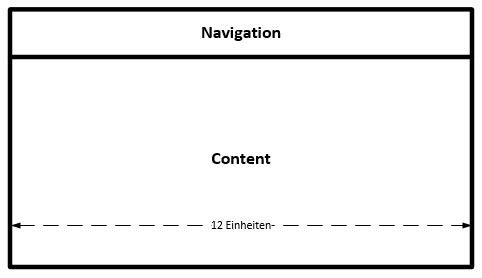
\includegraphics[scale=0.9]{../04_Realisierung/images/userinterface/seitenlayout_allgemein_large.png}
\caption{Seitenlayout Allgemein}
\end{figure}
Das Grid-System von Bootstrap teilt den sichtbaren Bereich in 12 Spalten auf. Jede Spalte besetzt immer $\frac{1}{12}$ der gesamten Fenstergrösse. Bootstrap verwendet folgende CSS Media-Queries für unterschiedliche Bildschirmtypen:
\begin{itemize}
\item Small Devices (min-width: 576px)
\item Tablets (min-width: 768px)
\item Desktops (min-width: 992px)
\item Large Desktops (min-width: 1200px)
\end{itemize}
Sämtlichen div-Containern wird angegeben, wieviele Spalten in welcher Bildschirmgrösse sie besetzen. Mit Bootstrap könnte dies folgendermassen aussehen: 
\begin{lstlisting}[language=html]
<div class="col-lg-6 col-md-6 col-sm-12 col-xs-12">
</div>
\end{lstlisting}
An diesem Beispiel besetzt dieser Div-Container auf mittelgrossen und grossen Desktops die Hälfte-, auf Tablets und Smartphones die gesamte Bildschirmbreite. Somit wird ein responsives Layout umgesetzt, dass die Applikation sowohl von mobilen-, als auch von Desktop Devices gut nutzbar ist.

\subsubsection{Navigation}
Bootstrap liefert eine ''default-navbar''. Sämtliche Navigationslinks (Home, Device, Discovery, Configurations, User Panel) befinden sich in der Navigationsleiste. Die Navigationsleiste besetzt in jeder Bildschirmgrösse die gesamte Breite.
\begin{lstlisting}[language=html]
<div class="col-lg-12 col-md-12 col-sm-12 col-xs-12">
</div>
\end{lstlisting}
\begin{figure}[H]
\centering
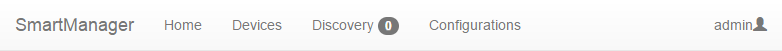
\includegraphics[scale=0.8]{../04_Realisierung/images/userinterface/navbar_lg.png}
\caption{Navigationsleiste gross}
\end{figure}

Da diese Navigationsleiste auf Smartphones schwierig zu bedienen ist, wird auf der kleinsten Bildschirmgrösse anstatt der normalen Links in der Navigation ein Hamburger-Button verwendet. Anfangs war dieser Button stark umstritten, mittlerweile wird er häufig eingesetzt, weshalb jedem Benutzer klar sein sollte, dass sich dahinter weitere Elemente befinden.
\begin{figure}[H]
\centering
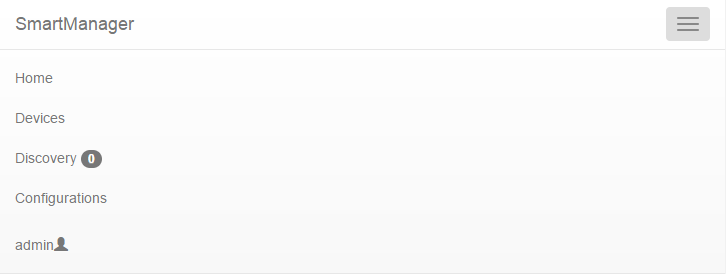
\includegraphics[scale=0.87]{../04_Realisierung/images/userinterface/navbar_xs.png}
\caption{Navigationsleiste xs}
\end{figure}

Die Navigationsleisten sind auf jeder Seite am oberen Bildschirmrand fixiert, sodass bei allfälligem Scrollen die Navigation trotzdem sichtbar bleibt.

Damit duplizierter Code auf jeder Seite verhindert wird, wird der gesamte HTML Code für die Navigation in ein eigenes JSP File ''menuFragment.jsp'' ausgelagert. Der Inhalt des JSP Files wird mittels 
\begin{lstlisting}[language=html]
<jsp:include page="../../views/menuFragment.jsp" />
\end{lstlisting}
serverseitig ins HTML gerendert.
\subsubsection{Content}
Der gesamte Content Bereich ist auf jeder Seite unterschiedlich gestaltet. Die gesamte Breite von 12 Spalteneinheiten kann verwendet werden.

\subsubsection{Asynchronous JavaScript and XML AJAX}
Damit bei der Kommunikation mit dem Server das User Interface nicht blockiert wird, werden bei sämtlichen Server-Calls AJAX verwendet. AJAX versendet Nachrichten vom Client an den Servern asynchron. Im ''success'' Attribut kann eine Callback-Funktion hinterlegt werden, welche bei erfolgreicher Antwort ausgeführt wird.

In dieser Applikation werden AJAX-Calls nach folgendem Schema ausgeführt:
\begin{lstlisting}
$.ajax({
	type : "GET/POST/DELETE",
	url : ctx + "/resource/method",
	success : function() {
		/*some callback code...*/
	},
	error : function(xhr, ajaxOptions, thrownError) {
		window.location.href = ctx + "/";
		alert(thrownError);
	}
});
\end{lstlisting}

Falls der Server mit einem Fehler antwortet, wird die Callback-Funktion im ''error''-Attribut ausgeführt. Der Benutzer wird dabei auf die Haupt-Seite umgeleitet und erhält eine Error-Meldung angezeigt.

\subsubsection{Bootbox}
An verschiedenen Stellen auf der Seite werden Pop-ups benötigt. In diesem Projekt wird die JavaScript Library ''Bootbox'' von Bootboxjs.com verwendet.

\begin{figure}[H]
\centering
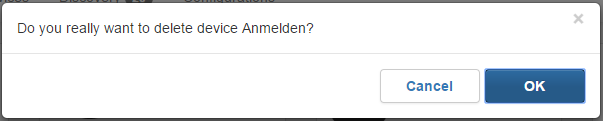
\includegraphics[scale=0.9]{../04_Realisierung/images/userinterface/bootbox.png}
\caption{Bootbox}
\end{figure}

Der JavaScript Code für die Erstellung und Verwendung der Bootbox ist leicht verständlich.

\begin{lstlisting}
bootbox.confirm({
	size : "large",
	title : "some title",
	message : content,
	callback : function(ok) {
		if (ok) {
			/*save, redirect etc.*/		
		}
	}
});
\end{lstlisting} 

Als ''message''-Attribut kann ein String oder auch HTML Code eingefügt werden.  Beim ''Callback''-Attribut kann eine Callback-Funktion hinterlegt werden. Diese wird ausgeführt, wenn das Pop-up Fenster geschlossen wird. Die if-Abfrage stellt sicher, dass der darinliegende Code nur ausgeführt wird, wenn ''OK'' auf geklickt wird.

\subsubsection{Google Maps API}
An verschiedenen Stellen auf der Seite werden Devices auf Google Maps Karten angezeigt. Dies gibt dem Benutzer eine schnelle Übersicht der Lokalitäten der IoT Devices.

Über die JavaScript-Funktion ''initMap()'' wird die (leere) Map geladen. Danach werden über die Funktion ''getLocations()'' die Locations der benötigten IoT Devices vom Server abgefragt. Über die ''insertLocations()''-Funktion werden die Punkte auf der Map eingezeichnet.

\subsection{Home}
Die Home-Seite dient als Einstiegspunkt und Übersichtsseite. Dem Benutzer sollen Informationen über die Applikation und die verwaltete Infrastruktur angezeigt werden.

\begin{figure}[H]
\centering
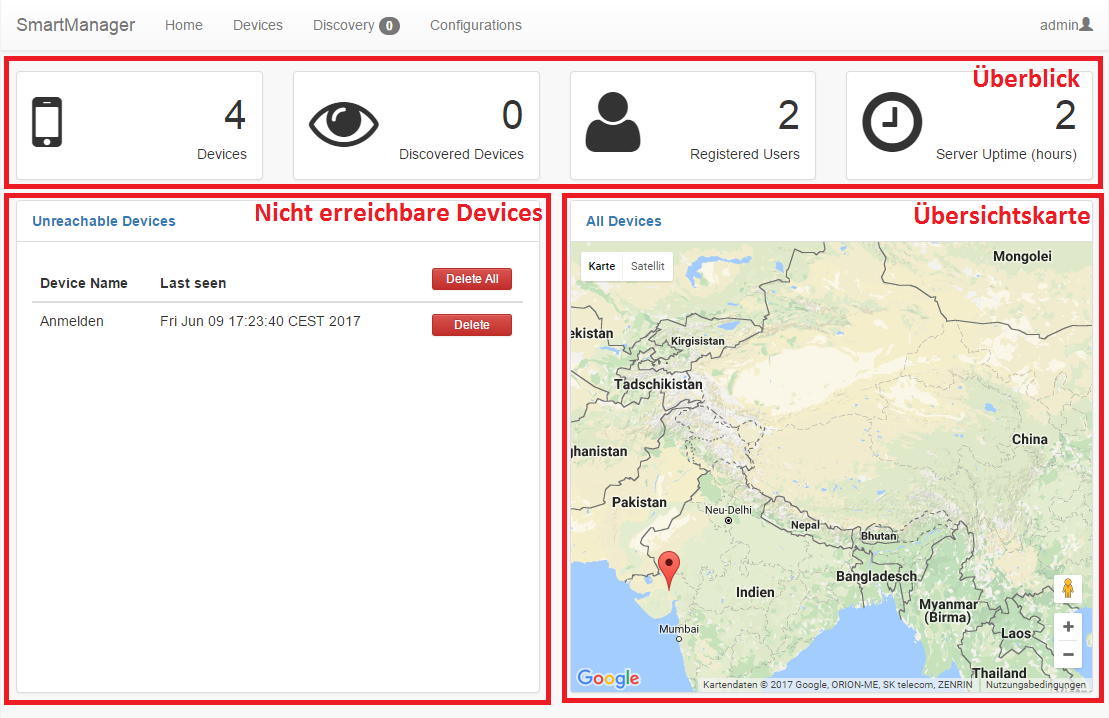
\includegraphics[scale=0.57]{../04_Realisierung/images/userinterface/home.png}
\caption{Dashboard}
\end{figure}

\subsubsection{Überblick}
In diesem Bereich werden dem Benutzer folgende vier Informationen auf den ersten Blick angezeigt:
\begin{itemize}
\item Gesamtanzahl erfasster Devices im System
\item Anzahl Devices im Discovery (noch nicht verwaltet)
\item Anzahl registrierter Benutzer
\item Server Uptime in Stunden
\end{itemize}

\subsubsection{Nicht erreichbare Devices}
Sind Devices nicht mehr erreichbar, muss dies dem Benutzer mitgeteilt werden. Hat sich ein Device mehr als 30 Minuten nicht mehr beim Server gemeldet, so erscheint es in dieser Tabelle. Klickt der Benutzer auf ''Delete'' respektive ''Delete All'', so werden die JavaScript Funktionen ''deleteUnreachableDevice(id, name)'' und ''deleteAllUnreachableDevices()'' ausgeführt. Über eine AJAX-Anfrage werden die entsprechenden Serverpfade aufgerufen.

\subsubsection{Übersichtskarte}
Auf dieser Übersichtskarte werden alle im Device gespeicherten Locations von IoT Devices angezeigt.

\subsection{Discovery}
\subsection{Devices und Groups}
\subsection{Configuration}




\section{Controllers}





\section{Services}





\section{LwM2M-Server}





\section{Database}





\section{Demo LwM2M-Client}
